\author{OTS}
\documentclass[14pt]{../../inc/mybib}

\setincpath{../../inc/}

\usepackage{bible_style}
\graphicspath{{../../assets/images/}}
\usepackage{header}
\usepackage{numprint}
% \usepackage{parskip}

\newcommand{\q}[1]{\blockquote{#1}}

\newenvironment{block}[1][]{%
  \vspace{1.5em}%
  \noindent\textbf{#1}\par%
  \vspace{0.0em}%
}{%
  \vspace{1em}%
}

\author{Lothar Schmid}

\begin{document}
\setlength{\baselineskip}{1.5\baselineskip}
\section{Babylon 1 Mose 11}

\subsection{Der Turmbau von Babel}
    \begin{block}[Einleitung]
    Babylon ist neben Jerusalem wohl die Stadt aus der Bibel, die am meisten bekannt ist. Ob Christen, Theologen oder Menschen, die nichts mit dem Christentum am Hut haben, kennen diese Geschichte mit dem Turmbau. Schon als Kinder haben wir diese Geschichte aus der Bibel gehört und es spannend gefunden, wie hoch der Turm wohl war. Babel ist aber auch für Zügellosigkeit und Sünde bekannt geworden. Babel wird auch im Zusammenhang mit Sprachen benutzt. Es gibt eine Babel-App, um Sprachen zu lernen, oder ein Babel-Programm in der Programmierwelt, mit dem man eine Programmiersprache in verschiedene Sprachversionen übersetzen kann.
    \end{block}
    \begin{block}
    Die Geschichte vom Bau des Turmes zu Babel finden wir in der Bibel in \bibleverse{IMos} {11:1-9}. Es ist eine kurze Geschichte, es ist jetzt auch nicht unbedingt eine spannende Geschichte, trotzdem hat diese Geschichte viele Maler, Gestalter, Dichter und Schriftsteller angeregt, darüber zu Schreiben, zu Malen und ihren Fantasien freien lauf zu lassen. 
    \end{block}

    \textbf{Wollen wir doch zusammen die Verse 1. Mose 11:1-9 einmal lesen.}
    
    \vspace{1em}
    \begin{block}
    Diese Geschichte findet zu einer Zeit statt, wo die Menschen noch eine gleiche Sprache und Wortschatz hatten.
    \begin{bibelbox}{SCHL}{1Mos}{11:1}
        Und die ganze Erde hatte eine einzige Sprache und dieselben Worte.
    \end{bibelbox}    
    In Vers 2 lasen wir, dass sie sich gemeinsam Richtung Westen auf den Weg gemacht haben. Im Land Schinar im heutigen Irak gelegen, liessen sie sich in einer Ebene nieder.    
    \begin{bibelbox}{SCHL}{1Mos}{11:2}
        Und es geschah, als sie nach Osten zogen, da fanden sie eine Ebene im Land Sinear und siedelten dort.
    \end{bibelbox}
    Wer war dieses Volk? Wann hat diese Völkerwanderung stattgefunden? Wenn wir ein Kapitel vorher die Verse  \bibleverse{IMos} (10:7-8) aufschlagen, finden wir dort einen detailierten Stammbaum von Noah. Wir wissen, dass Noah und seine Söhne noch zu den Menschen gehörten, die sehr alt wurden. Wie lange sie lebten finden wir im Kapitel 11 in den Versen 10-26, dort ist der Stammbaum von Sem bis Terach dem Vater von Abraham aufgelistet. Ich habe mir die Mühe gemacht, diese Alter in einem Balkendiagramm darzustellen und dann sieht man, dass Abraham nur wenige Jahre nach dem Tod von Noah auf die Welt kam. 

    \begin{figure}[ht]
    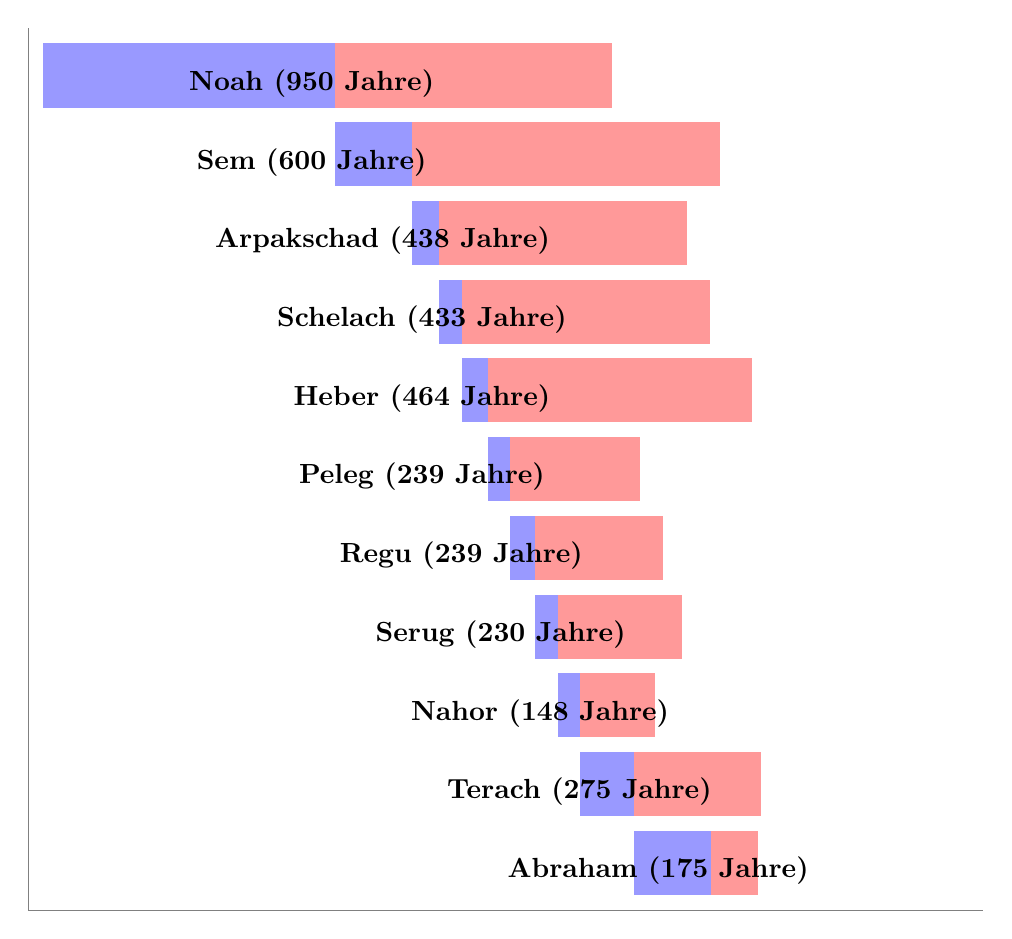
\begin{tikzpicture}
        \draw[gray] (0,0) -- (0mm, 112mm);
        %Noah 500-450 (0 - 93.6)
        \filldraw[blue!40] (2mm,110mm) rectangle(39mm,102mm);
        \filldraw[red!40] (39mm,110mm) rectangle(74.1mm,102mm) node at (36mm, 102mm) [right, above, black]{\textbf{Noah (950 Jahre)}};
        
        %Sem 100-500 (0 - 93.6)
        \filldraw[blue!40] (39mm, 100mm) rectangle(48.8mm,92mm);
        \filldraw[red!40] (48.8mm,100mm) rectangle(87.8mm,92mm) node at (36mm, 92mm) [right, above, black]{\textbf{Sem (600 Jahre)}};
        
         %Arpakschad 35-403 (15.6 - 62.4)
         \filldraw[blue!40] (48.8mm,90mm) rectangle(52.2mm,82mm);
        \filldraw[red!40] (52.2mm,90mm) rectangle(83.6mm,82mm) node at (45mm, 82mm) [left, above, black] {\textbf{Arpakschad (438 Jahre)}};
        
        %Schelach 30-403 (15.6 - 62.4)
        \filldraw[blue!40] (52.2mm,80mm) rectangle(55.1mm,72mm);
        \filldraw[red!40] (55.1mm,80mm) rectangle(86.5mm,72mm) node at (50mm, 72mm) [right, above, black] {\textbf{Schelach (433 Jahre)}};
        
        \filldraw[blue!40] (55.1mm,70mm) rectangle(58.4mm,62mm);
        \filldraw[red!40] (58.4mm,70mm) rectangle(91.9mm,62mm) node at (50mm, 62mm) [right, above, black] {\textbf{Heber (464 Jahre)}};
        
        \filldraw[blue!40] (58.4mm,60mm) rectangle(61.3mm,52mm);
        \filldraw[red!40] (61.3mm,60mm) rectangle(77.6mm,52mm) node at (50mm, 52mm) [right, above, black] {\textbf{Peleg (239 Jahre)}};
        
        \filldraw[blue!40] (61.3mm,50mm) rectangle(64.4mm,42mm);
        \filldraw[red!40] (64.4mm,50mm) rectangle(80.6mm,42mm) node at (55mm, 42mm) [right, above, black] {\textbf{Regu (239 Jahre)}};
        
        \filldraw[blue!40] (64.4mm,40mm) rectangle(67.4mm,32mm);
        \filldraw[red!40] (67.4mm,40mm) rectangle(83.0mm,32mm) node at (60mm, 32mm) [right, above, black] {\textbf{Serug (230 Jahre)}};
        
        \filldraw[blue!40] (67.4mm,30mm) rectangle(70.2mm,22mm);
        \filldraw[red!40] (70.2mm,30mm) rectangle(79.5mm,22mm) node at (65mm, 22mm) [right, above, black] {\textbf{Nahor (148 Jahre)}};
        
        \filldraw[blue!40] (70.2mm,20mm) rectangle(77mm,12mm);
        \filldraw[red!40] (77mm,20mm) rectangle(93.0mm,12mm) node at (70mm, 12mm) [right, above, black] {\textbf{Terach (275 Jahre)}};

        \filldraw[blue!40] (77mm,10mm) rectangle(86.8mm,2mm);
        \filldraw[red!40] (86.8mm,10mm) rectangle(92.6mm,2mm) node at (80mm, 2mm) [right, above, black] {\textbf{Abraham (175 Jahre)}};
        \draw[gray] (0,0) -- (\textwidth, 0mm);
    \end{tikzpicture}
    \caption{Lebensjahre von Noah bis Abraham}
    \label{balken_alter}
\end{figure}
    
    Es gibt also Noah --> Ham --> Kusch und Kusch war der Vater von Nimrod.
    \begin{bibelbox}{SCHL}{1Mos}{10:9}
        Er war ein gewaltiger Jäger vor dem HERRN; daher sagt man: Wie Nimrod, ein gewaltiger Jäger vor dem HERRN!
    \end{bibelbox}
    Wenn wir jetzt beachten, dass Nimrod die 3. Generation nach Noah ist, wurde Nimrod sicher auch um die 500 Jahre alt. Jede Generation starb immer jünger. 
\end{block}
\begin{block}
    So gab es in der Bevölkerung Menschen die Uralt waren und solche die jung starben. Wir müssen uns das so vorstellen:  Du lebst in deinem Dorf und in diesem Dorf gibt es einen Bürgermeister der schon bei deinem Urgrossvater, Grossvater, Vater und aktuell immer noch Bürgermeister ist. Jetzt bist du und alt stirbst bald aber der Bürgermeister lebt noch fröhlich weiter. Würden diesem Bürgermeister nicht auch übersinnliche Kräfte zugeschrieben? 
\end{block}
\begin{block}
    Von Nimrod wird gesagt, dass er der erste Gewaltherrscher war. Es gibt auch ausserbiblische Schriften wie zum Beispiel der Gilga-Mesh Epos wo die Könige mehre tausend Jahre alt wurden. Ist wohl übertrieben, aber zeigt, dass auch ausserbiblische Quellen von Menschen spricht, die sehr alt wurden. Nimrod war also der Machthaber zu der Zeit und versammelt das Volk um sich. Er nun will, um seine Macht zu festigen, eine grosse Stadt mit einem riesigen Turm bauen.
\end{block}
\begin{block}
    Nimrod kannte den Gott der Bibel sicher noch. Sein Grossvater war ja mit auf der Arche. Er wusste, dass dieser Gott eine Sindflut ausgelöst hat und ausser Noah und seine Familie alles getötet hat, was an Land lebte. Nimrod war ein Machtherrscher, er wollte sich verewigen, er wollte sich ein Denkmal setzen. Er ist der aktuelle Machthaber und fühlt sich diesem unsichtbaren Gott überlegen.
\end{block}
\begin{block}
    Im Vers 5 lesen wir wie Gott vom Himmel herunterkommt und sich das ganze treiben anschaut. Wieso war Gott nicht zufrieden mit dem, was er sah? Ist Gott dagegen, dass die Menschen Stätte und Türme bauten? Nein, das glaube ich nicht. Gott hatte Noah einen genauen Auftrag gegeben. Noah hat das wohl nicht richtig seinen Nachkommen kommuniziert denn in \bibleverse{1Mos}(9:1)
    \begin{bibelbox}{SCHL}{1Mos}{9:1}
        Und Gott segnete Noah und seine Söhne und sprach zu ihnen: Seid fruchtbar und vermehrt euch und füllt die Erde!
    \end{bibelbox}    
    
    Da steht nicht \q{baut euch eine schöne Stadt und  bleibt einmütig zusammen}, sondern, \q{verteilt euch auf der ganzen Welt und bearbeitet diese.} Gottes Anweisung wurde ignoriert und das Schicksal in die eigenen Hände genommen. 
\end{block}
\begin{block}
    Menschen im Team können viel leisten. Gemeinsame Sprache, gemeinsamer Austausch, das ist die Voraussetzung für Fortschritt. Das sehen wir daran, dass sie jetzt nicht mehr Steine für den Bau benutzten, sondern Ziegel brannten. Mit Ziegel ist es leichter und einfacher einen TUrm zu bauen. \textbf{Aber die Zeit war noch nicht reif.} Das war nicht Gottes Plan.
\end{block}
\begin{block}
    Roger Liebi hat da ein interessanter Gedanken formuliert. Die Menschen damals waren alles andere als dumm. Gemeinsam im Team konnten sie viel leisten. Der Fortschritt wäre für die Welt zu schnell gekommen. Liebi meinte dazu: \enquote{hätte Gott dem nicht ein Riegel vorgeschoben, hätten die Römer schon mit Raketen Krieg geführt.}
\end{block}
\begin{block}
    Darum hat Gott eingriffen. Er hat einfach jeder Sippe ihre eigene Sprache gegeben. Ohne Kommunikation war die Teamarbeit schnell beendet. Die einzelnen Sprachgruppen sind dann weggezogen und haben sich auf der ganzen Welt verteilt. Genauso wie es Gott immer wollte.
    Darum gibt es im Kapitel 10 bei den Nachkommen Noahs immer wieder der Zusatz:
    \begin{bibelbox}{SCHL}{1Mos}{10:5.20.31}
        Das sind die Söhne Hams nach ihren Geschlechtern, Sprachen, Ländern und Völkern.
    \end{bibelbox}    
    
    Die einzelnen Sippen haben also ihre Sachen gepackt und sind auf Wanderschaft. Was zurück blieb, war ein unfertig gebauter Turm.
\end{block}
\begin{block}
    Ist jetzt damit das Thema Turmbau beendet? Ende der Predigt? Nein leider noch nicht. Kommen wir zum Volk Israel und schauen uns dort an wo das Volk Isreal ihre Türme gebaut hat.
    
    \section{Turmbau von Israel}
    Kommen wir zum Teil zwei dieser Predigt. Ich habe diese Predigt in 4 Teile aufgeteilt. Jeder Teil zeigt eine Epoche in der Heilsgeschichte Gottes. Kommen wir jetzt zum Volk Gottes, zu Israel.
\end{block}
\begin{block}
    Wir haben jetzt also eine Stadt mit dem Namen Babylon und einen halbfertigen Turm. Ein im Jahr 1913 ausgegrabenes Fundament 80\,km südlich von Bagdad wird diesem Turm zugeteilt, einen sogenannten Zikkurat. Verlassen wir aber jetzt mal diesen Turm und kommen zu Abraham.
\end{block}
\begin{block}
    Abraham wohnte in Ur und wurde mit 75 Jahren von Gott auserwählt, der Gründer von seinem Volk zu werden. 
    \begin{bibelbox}{SCHL}{1Mos}{12:1}
        Der HERR aber hatte zu Abram gesprochen: Geh hinaus aus deinem Land und aus deiner Verwandtschaft und aus dem Haus deines Vaters in das Land, das ich dir zeigen werde!
    \end{bibelbox} 

    Klare Anweisung, aber nicht leicht unzusetzen mit 75, aber die Anweisung war klar. Oder? Abraham hat aber sein eigenes Türmchen gebaut. Obwohl Gott gesagt hat, \enquote{geh aus deiner Verwandtschaft} nahm er Lot mit. In der späteren Geschichte lesen wir dann, von den Problemen die mit Lot auftauchten. In \bibleverse{1Mos}(14:) Die Entführung und Rettung von Lot und später \bibleverse{1Mos}(19:) Probleme in Sodom und Gomorra, was zum Tod seiner Frau \bibleverse{1Mos}(19:24) und der Inzucht mit seinen Töchtern in \bibleverse{1Mos}(19:30-38) führte.
\end{block}
\begin{block}
    Seht ihr, worauf ich hinaus will? Gott gibt eine Anweisung und wir denken uns, wir seien schlauer als er und können unsere eigenen Türme in unserem Leben bauen. Wie viele Türme habe ich wohl, in meinem kurzen Glaubensleben schon gebaut?
\end{block}
\begin{block}
    Gehen wir aber weiter mit der Suche nach Türmen. Die Probleme in der Wüstenwanderung kennen wir. Das Volk kam in seiner Wanderung zum gelobten Land an die Grenze dieses Landes. Gott sagte Moses, er solle Kundschafter ausschicken und das Land erkunden. Zu lesen in \bibleverse{4Mos}(13:) Das wurde gemacht und nach 40 Tagen kamen die Kundschafter zurück und erzählten von ihren Erlebnissen. Gott hat ihnen versprochen sie sicher in das Land führen, aber sie glaubten ihm nicht. Zur Strafe für ihre Rebellion mussten sie jetzt 40 Jahre durch die Wüste wandern. Oh, da haben sie wohl geschnallt, dass die Rebellion gegen den Einmarsch ins Gelobte Land \bibleverse{IIIMos}(14:) nicht so gut war. Um ihr vergehen wiedergutzumachen, fingen sie an ihren eigenen Turm zu bauen und ihre Zukunft in die eigene Hand zu nehmen. Moses warnt sie davor, ihr vorhaben auszuführen. Sie hörten aber nicht auf Moses und zogen stur in das Land und wurden von den Amalekiter und den Kanaaiter wieder zurückgejagt. Fertig war der Bau vom eigenen Turm.
\end{block}
\begin{block}
    Auch im Buch Richter finden wir ein schönes Beispiel. Nämlich Gideon. In \bibleverse{Ri}(6:11-24) lesen wir vom Erlebnis, welches Gideon mit dem Engel des Herrn hatte. Später lesen wir in \bibleverse{Ri}(6:38-40) wie Gott Gideon den Beweis seiner Existenz, anhand eines Vlies und mit Tau bewies. Auch \bibleverse{Ri}(7:) der Sieg über die Midianiter, beweist eindrücklich Gottes Existenz. Eigentlich sollte doch jetzt Gideon überzeugt sein. Aber Gottes Gnade genügt ihm nicht. Gideon hat aus dem Volk Gold gesammelt und liess sich daraus ein Ephod also ein Priestergewand ferigen. So lesen wir in:
    \begin{bibelbox}{SCHL}{Ri}{8:27}
        Und Gideon machte ein Ephod daraus und stellte es in seiner Stadt auf, in Ophra. Und ganz Israel hurte ihm dort nach. Und das wurde zum Fallstrick für Gideon und sein Haus.
    \end{bibelbox} 
    Sein eigenmächtiges Handeln wurde zum Fallstrick für seine Sippe. Das zeigt, dass nicht mal der persönliche Kontakt mit Gott vor dem Bau eigener Türme schützt.
\end{block}
\begin{block}
    Gehen wir weiter zu Saul. Sein persönlicher Turmbau, der ins Verderben führen sollte. Saul wurde von Gott als den ersten König auserwählt. Auch das ist so ein Turmbau. Gott wollte der König von Israel sein. Das reichte aber dem Volk Israel nicht. Obwohl Gott schon in \bibleverse{5Mos}(17:14-20) vor einem König warnte, wollte sie trotzdem einen eigenen König. Wenigstens haben sie die Anweisung beachtet, dass nur Gott einen König auswählen soll. Saul wurde also König und sollte eigentlich nur Gottes Anweisungen beachten und ausführen, die ihm von Samuel überbracht wurden. In \bibleverse{ISamuel}(15:) lesen wir, wie Saul sich nicht an die Anweisungen hielt, sondern anfing seinen eigenen Turm zu bauen. Gott sagt zu Saul:
    \begin{bibelbox}{SCHL}{1Sam}{15:3}
        So ziehe nun hin und schlage Amalek, und vollstrecke den Bann an allem, was er hat, und schone ihn nicht; sondern töte Männer und Frauen, Kinder und Säuglinge, Rinder und Schafe, Kamele und Esel!
    \end{bibelbox}
    Saul zog in den Krieg gegen Amalek und dann heisst es:
    \begin{bibelbox}{SCHL}{1Sam}{15:9}
        Aber Saul und das Volk verschonten Agag und die besten Schafe und Rinder und das Vieh vom zweiten Wurf und die Mastschafe und alles, was wertvoll war, und sie wollten den Bann an ihnen nicht vollstrecken; alles Vieh aber, das wertlos und schwächlich war, an dem vollstreckten sie den Bann.
    \end{bibelbox}
    Saul hat gegen Gottes Gebot gehandelt. Der Vers 21 erinnert mich wieder an Adam und Eva. Auch da schiebt Eva die Schuld auf andere. So lesen wir folgende Aussage von Saul
    \begin{bibelbox}{SCHL}{1Sam}{15:21}
        Aber das Volk hat von der Beute genommen, Schafe und Rinder, das Beste des Gebannten, um es dem HERRN, deinem Gott, in Gilgal zu opfern!
    \end{bibelbox}
    Gott will gehorsam und keine Opfergaben. Wenn man Gott nicht gehorcht, dann muss man auch mit den Folgen zurechtkommen. Ist heute nicht anders, wie zu jener Zeit. Nur der Gehorsam zu Gott bringt auf langer Sicht Frieden mit sich und dem eignen Umfeld. Dies musste nun auch Saul erfahren. Der Prophet Samuel überbrachte ihm die Worte des \herr N für sein ungehorsam.    
    \begin{bibelbox}{SCHL}{1Sam}{15:22-23}
        Samuel aber sprach: Hat der HERR dasselbe Wohlgefallen an Schlachtopfern und Brandopfern wie daran, dass man der Stimme des HERRN gehorcht? Siehe, Gehorsam ist besser als Schlachtopfer, und Folgsamkeit besser als das Fett von Widdern! Denn Rebellion ist wie die Sünde der Wahrsagerei, und Widerspenstigkeit ist wie Abgötterei und Götzendienst. Weil du das Wort des HERRN verworfen hast, so hat er dich auch verworfen, dass du nicht mehr König sein sollst.
    \end{bibelbox} 
    Von da an war sein Königtum nur noch ein Trümmerhaufen. Der Aussgang Saul's kennt ihr. Er litt an Verfolgungswahn und führte ein verbittertes Leben.
\end{block}
\begin{block}

    Es sind jetzt nicht nur die einzelne Person in Israel die angefangen haben Türme zu bauen. Das Volk wollte einen König, Gott war nicht mehr gut genug. Gott hat schon in \bibleverse{VMos}(1:) davor gewarnt einen König aus dem Volk zu erwählen. Nicht weil er eifersüchtig war, oder Angst hatte das ihm jemand den Posten streitig macht. Sondern, er wusste das der Mensch machtgierig und brutal ist.
    
    Sobald Menschen an der Macht sind, verändern sie sich. Schauen wir uns noch ein Beispiel an, und zwar der König Ussijas. Ussija war 52 Jahre lang König von Judäa. Über ihn lesen wir in \bibleverse{2Chronik}(25:4-5), dass er tat, was der \herr{} wollte. 
    \begin{bibelbox}{SCHL}{2Chronik}{26:4}
        Und er tat, was recht war in den Augen des HERRN, ganz wie es sein Vater Amazja getan hatte
    \end{bibelbox} 
    Gott half ihm in seinen Regierungsjahren sich gegen die Philister, Abraber und Ammoniter zu Behaupten und wurde bis nach Ägypten berühmt. Er baute Türme (richtige Türme), bewässerte die Wüste und legte Gärten in den Bergen an. Es heisst in Ver 15b
    \begin{bibelbox}{SCHL}{2Chronik}{26:15}
        \dots so verbreitete sich sein Ruhm weithin, weil ihm wunderbar geholfen wurde, bis er sehr stark wurde.
    \end{bibelbox} 

    Und dann, in Vers 16
    \begin{bibelbox}{SCHL}{2Chronik}{26:16}
        Als er aber stark geworden war, überhob sich sein Herz zu seinem Verderben, und er versündigte sich an dem HERRN, seinem Gott, indem er in die Tempelhalle des HERRN ging, um auf dem Räucheraltar zu räuchern.
    \end{bibelbox} 
    Es reichte ihm nicht König zu sein. Er wollte mehr. Er fing an, an seinem persönlichen Turm zu bauen. Er wollte auch noch \underline{der} Priester sein. Wir wissen ja, dass Gott die Regierung und das Priestertum strikte getrennt hat. 
    \enquote{Hi, was bin ich doch für ein Held! Wenn ich als König schon so toll bin, dann sicher auch im Tempel als Priester.} 80 Priester wollten ihn zur Vernunft bringen. Er wurde aber zornig und wollte mit der Räucherpfanne weiter räuchern. Da setzte Gott diesem Turmbau ein Ende. Ussija bekam Aussatz und war im Rest seines Lebens in quarantäne. Quasi ein von Gott ausgesprochener Hausarrest.
\end{block}
\begin{block}
    Nachdem die aus dem Südreich aus dem Exil von Babilon zurück nach Israel und Jerusalem kamen, bauten sie den Tempel wieder auf. Diese Geschichte lesen wir in Nehemia und Esra. Durch den Einsatz dieser beiden Männer blühte Israel langsam wieder auf. Nie mehr so wie früher aber, sie fingen wieder mit den Opfer an und fingen an die Schrift zu studieren. Es wurden Schriftgelehrte ausgebildet, welche die Menschen in der Schrift unterwiesen. 
    
    Nach den Propheten, in der Zeit der Makkabäer, enstand die Gruppe der Pharisäer. Ich nehme an, dass diese zu Beginn es sicher gut meinten. Sie studierten die Schriften. Sie wussten aus der Geschichte, wie schlecht es gehen kann, wenn man die Gebote Gottes missachtet. Am Anfang meinten sie es sicher gut. Sie wollten verhindern, dass das Volk wieder anfängt ihren Turm zu bauen. Aber als diese Gruppe ihre Macht über das Fussvolk erkannten, fingen auch sie mit dem Turmbau an. Sie verschärften die Gesetze, bereicherten sich an der Bevölkerung und spielte sich als die wahren Gläubigen auf.
    
    In den Evangelien lesen wir wie Jesus zu diesen Pharisäer stand. Jesus hat diese Gruppe scharf kritisiert:  Schlangenbrut, Otternbrut und Heuchler hat er diese Religionselite genannt und Blinde die Blinde führen.
    \begin{bibelbox}{SCHL}{Matt}{15:14}
        Lasst sie; sie sind blinde Blindenleiter! Wenn aber ein Blinder den anderen leitet, werden beide in die Grube fallen.
    \end{bibelbox} 
    Der Turmbau dieser Gruppe endete schrecklich. Einmal zum Tod des Herrn Jesu und dann später auch zur Zerstörung von Jerusalem durch die Römer mit vielen Millionen Toten. 
    
    \textbf{Und jetzt? Jetzt hat aber der Turmbau sicher ein Ende. Oder?}
\end{block}

    \subsection{Der Turmbau der Gemeinde}
    Schauen wir mal weiter. Kommen wir zum dritten Teil:  der Gemeinde.
    \begin{block}
    Als Jesus unter uns weilte, gab er uns genaue Anweisungen, wie wir das Heil erlangen können und wie wir ein von Gott wohlgefälliges Leben führen. Diese Anweisungen hat uns der \herr{} in den Evangelien mitgegeben, aber vor allem in den Lehrbriefen. Die Briefe zeigen uns auf, wie wir unser Christenleben leben sollten.
    Jesus hat uns gesagt wie wir von unseren Sünden befreit werden und wie wir die Gnade Gottes und das ewige Leben erlangen können. Zum Beispiel
    \begin{bibelbox}{SCHL}{Joh}{11:25-26}
        Jesus spricht zu ihr: Ich bin die Auferstehung und das Leben. Wer an mich glaubt, wird leben, auch wenn er stirbt;und jeder, der lebt und an mich glaubt, wird in Ewigkeit nicht sterben. Glaubst du das?
    \end{bibelbox} 
    \begin{bibelbox}{SCHL}{Joh}{1:12-13}
        Allen aber, die ihn aufnahmen, denen gab er das Anrecht, Kinder Gottes zu werden, denen, die an seinen Namen glauben;
        die nicht aus dem Blut, noch aus dem Willen des Fleisches, noch aus dem Willen des Mannes, sondern aus Gott geboren sind.
    \end{bibelbox} 
    Das ist \textbf{\underline{die gute Botschaft.}}
    Eigentlich klar oder? Ist es so missverständlich? Oder ist es einfach zueinfach? Wie heisst es hier im Wallis so schön: \enquote{Was nigs kostut, isch nit brüchusch wärt.} Jesus, unser Herr, gab uns auch eine Anweisung, was wir jetzt mit diesem neu erlangten Leben tun sollen:
    \begin{bibelbox}{SCHL}{Mk}{16:15}
        Und er sprach zu ihnen: Geht hin in alle Welt und verkündigt das Evangelium der ganzen Schöpfung!
    \end{bibelbox} 
    Auch das sind doch klare Worte oder?
\end{block}

    Am Anfang der Kirchengeschichte klappte es ja auch.
\begin{block}
    Ab \bibleverse{Apg}(2:14) steht die gewaltige Evangelisationsrede des Apostel Petrus. Am Ende heisst es:
    \begin{bibelbox}{SCHL}{Apg}{2:40-41}
        Und noch mit vielen anderen Worten gab er Zeugnis und ermahnte und sprach: Lasst euch retten aus diesem verkehrten Geschlecht! Diejenigen, die nun bereitwillig sein Wort annahmen, ließen sich taufen, und es wurden an jenem Tag etwa 3 000 Seelen hinzugetan.
    \end{bibelbox} 
    3000 Seelen haben sich zu Jesus bekehrt. Und das nur wegen der Rede von Petrus?
    
    Lernt doch mal diese Rede auswendig, geht dann zum nächsten Fussball WM Finale ins Stadion und gebt die Predigt von Petrus über das Mikrofon an die Zuschauer weiter. Was denkt ihr wieviele sich bekehren werden? Unser Auftrag ist nicht Menschen zu bekehren. Das macht Gott. Unser Auftrag ist die Gute Botschaft zu verkünden.
\end{block}
\begin{block}
    Aber irgendwie ist das für uns Menschen zu einfache. Einfache nur Glauben, Vertrauen und von Gott reden? Mehr nicht? Ich muss doch irgendwas tun.
\end{block}
\begin{block}
    So begann der Turmbau schon früh in der Christenheit. Sehr früh wurden diverse Rituale und diverse Bedingungen eingeführt, die erfüllt werden müssen um das Heil zu erlangen. 
    Paulus spricht im Galater Brief die Beschneidung an.
    \begin{bibelbox}{SCHL}{Gal}{5:6}
        denn in Christus Jesus gilt weder Beschneidung noch Unbeschnittensein etwas, sondern der Glaube, der durch die Liebe wirksam ist.
    \end{bibelbox}
    Er hätte das nicht erwähnt, wenn es in den Gemeinden nicht disskutiert worden wäre. Das ist so ein typischer Stein den man benutzen kann um einen Turm zu bauen. Wir müssen immer differenzieren zwischen, das Heil erlangen und dem Leben mit diesem Heilsaussichten. Das erste bekommen wir aus Gnade, das zweite machen wir aus Dankbarkeit.

    Im ersten Konzil wurde besprochen wie gross und schwer so ein Stein sein sollte. Wenn ein Turm gebaut werden muss, so versuchten die Apostel in diesem Konzil diesen Ziegel der dort gebrann wurde, so klein wie möglich zu halten. Keine Unmoral und kein Blut essen. 
    \begin{bibelbox}{SCHL}{Apg}{15:20}
        sondern ihnen nur schreiben soll, sich von der Verunreinigung durch die Götzen, von der Unzucht, vom Erstickten und vom Blut zu enthalten.
    \end{bibelbox}
    Dieses Konzil war aber nicht das letzte, sondern es folgten 7 weitere Konzile vor der Kirchenspaltung in die Ostkirche und die Westkirche. Verschiedenen Gruppierungen waren sich nicht einig, wie der Turm auszusehen hat und so errichttete jeder seine eigene Baustelle. Die Türme werden heute \enquote{Die Orthodoxe Kirche} und \enquote{Die Katholische Kirche} genannt. Es folgten 21 weiter Konzile in der römisch-katholischen Kirche. Nebenbei fanden noch unzählige regionale Synoden statt.
    
    Bei jedem Konzil wurde wieder ein Stein mehr auf den Turm gesetzt, um zu versuchen, unabhängiger von Gott zu werden. Waren es am Anfang noch Theme wie das Glaubensbekenntnis(325~n.\,Chr), die Dreifaltigkeit(381~n.\,Chr)) oder ob Jesus ganz Gott oder Mensch ist(451~n.\,Chr)), wurdes es später Themen wie die Sakramente (1563~n.\,Chr)), Unfehlbarkeit des Papstes(1869~n.\,Chr)), Ökumene (1965~n.\,Chr)). Natürlich gab es noch mehr Themen, aber wir sehen hier an den Hauptthemen, dass der Mensch immer mehr Gott spielen möchte. Er will die Macht.
    Irgendwo habe ich gelesen, dass geprüft wird, ob es nicht auch reichen würde an Maria zu glauben um das Heil zu erlangen.
    
    Es spitzt sich also immer mehr zu. Wann wird Gott diesen Turmbau zerstören?
\end{block}
\begin{block}
    Aber nicht nur die katholische Kirche, sondern auch die evang. Kirche hat sich nach der Reformation wieder schnell mit dem Bau ihres eigenen Turms begonnen.
    Luther und Zwingli haben sich wegen der Taufe und dem Abendmahl gestritten. Calvin kam dazu mit seiner Heilstheorie. Die Wiedertäufer wurden als Kezer verbrannt. Es entstand wieder eine Machtstruktur. Auch heute reicht der Evangelischen Kirche das Wort Gottes nicht mehr. Und weil das einer Gruppe nicht passte, enstanden daraus die Freikirchen.\\
    Die Freikirchen wollten wieder zurück zum klaren Wort Gottes und haben eigene Gemeinden ins Leben gerufen. Der Turmbau ist aber immer noch nicht gebannt und läuft tapfer weiter, auch in den Freikirchen. Dürfen Frauen predigen? Lange Hosen, kurze Hosen? Haare bedecken oder nicht? Sabbath einhalten oder den Sonntag? Das sind Themen, über die man Stunden lang disskutiert und dabei vergisst was Jesus eigentlich gesagt hat. Wissen wir es noch? Haben wir die Worte vor Augen, wenn wir gläubigen und ungläubigen Mitmenschen begegnen? Beurteilen wir zuerst die Personen die in unser Gemeinde kommen wollen, ob diese in unseren eigends gebauten Turm passen? Wie reagieren wir, wenn jemand an unserem Turm, unserer geliebten Gemeindehülle, wackelt? Vielleicht sind ja die Kritiken angebracht. Wir haben aber lieber, wenn unsere Schäfchen brav Zeigel streichen um hoch hinaus zu kommen.
    Lesen wir nochmals Jesus Anweisung und seinen Auftrag:
    \begin{bibelbox}{SCHL}{Joh}{11:25-26}
        Jesus spricht zu ihr: Ich bin die Auferstehung und das Leben. Wer an mich glaubt, wird leben, auch wenn er stirbt;und jeder, der lebt und an mich glaubt, wird in Ewigkeit nicht sterben. Glaubst du das?
    \end{bibelbox} 
    \begin{bibelbox}{SCHL}{Joh}{1:12-13}
        Allen aber, die ihn aufnahmen, denen gab er das Anrecht, Kinder Gottes zu werden, denen, die an seinen Namen glauben;
        die nicht aus dem Blut, noch aus dem Willen des Fleisches, noch aus dem Willen des Mannes, sondern aus Gott geboren sind.
    \end{bibelbox}     
    \begin{bibelbox}{SCHL}{Mk}{16:15}
        Und er sprach zu ihnen: Geht hin in alle Welt und verkündigt das Evangelium der ganzen Schöpfung!
    \end{bibelbox} 
    Heute sind es Themen wie Klimawandel, Queer, Ökumene, also weltliche Themen die oft in den Gemeinden wichtiger sind, als die Worte Jesus. Denken wir daran, dass jeder Mensch, der ohne Jesus Christus im Herzen stirbt, in den Feuersee geworfen wird, egal ob die Welt gut ist, oder ob wir tollerant sind. 
    \begin{bibelbox}{SCHL}{Mk}{16:16}
        Wer glaubt und getauft wird, der wird gerettet werden; wer aber nicht glaubt, der wird verdammt werden.
    \end{bibelbox} 
\end{block}
    \subsection{Mein privater Turmbau}
\begin{block}
    Wenn wir zurückblicken auf die Türme, die wir gesehen haben, um was ging es den Erbauer eigentlich? Richtig, es geht um Stolz, Gier und Macht. Wir lassen uns nicht gerne irgenwas vorschreiben. Wir wissen alles besser. Jesus sagt in  
    \begin{bibelbox}{SCHL}{Matt}{11:28-30}
        Kommt her zu mir alle, die ihr mühselig und beladen seid, so will ich euch erquicken!
        Nehmt auf euch mein Joch und lernt von mir, denn ich bin sanftmütig und von Herzen demütig; so werdet ihr Ruhe finden für eure Seelen!
        Denn mein Joch ist sanft und meine Last ist leicht.
    \end{bibelbox}  
    Wir wollen aber kein leichtes Joch. Wir wollen ein schweres, wir wollen was leisten und wenn das Joch von Gott zu leicht ist, dann streichen wir Ziegel, mischen Zement und fangen an, auf dem Bau zu arbeiten. Immer ein seeliges Lächeln, ein Jahr lang kein GD auslassen, 3mal im Jahr die Bibel durchlesen und und und\dots Ziegel auf Ziegel \dots
\end{block}
\begin{block}
    Das will Jesus nicht, das verlangt er nicht von uns. Er will keine verbissenen Christen, die auf biegen und brechen versuchen ihm zu gefallen. Er will, dass wir ehrlich im Herzen sind und ihn lieben und an ihn glauben. Das ist alles. Mehr will er nicht. Wenn wir Jesus lieben und ihm dankbar sind für das, was er für uns am Kreuz gemacht hat, dann versuchen wir doch automatischen, Sachen zu vermeiden die ihn verletzen können. Ist doch zu Hause auch so. Wenn ich meinen Ehepartner liebe und dieser nicht mag wenn ich meine Suppe schlürfe, dann setzte ich mich doch nicht an Tisch und fange an zu schlürfen. Sondern ich setze mich hin und versuche mein Suppe anständig, ohne Geräusche zu essen. Sollte es doch mal passieren, dass es laut wurde, kann ich mich ja entschuldigen und ohne schlürfen weiter essen, ohne das dabei die Ehe gleich zubruch geht. Wenn ich aber extra Schlürfe beim Suppenessen, sitze ich plötzlich alleine vor meinem Suppenteller.

    Übertragen, wenn ich weiter in der Sünde verharre, dann kann der hl. Geist nicht mehr in mir wirken und mein Leben wird bitter.
\end{block}
\begin{block}
    Lesen wir nochmals was Jesus gesagt hat:
    \begin{bibelbox}{SCHL}{Joh}{11:25-26}
        Jesus spricht zu ihr: Ich bin die Auferstehung und das Leben. Wer an mich glaubt, wird leben, auch wenn er stirbt;und jeder, der lebt und an mich glaubt, wird in Ewigkeit nicht sterben. Glaubst du das?
    \end{bibelbox} 
    \begin{bibelbox}{SCHL}{Joh}{1:12-13}
        Allen aber, die ihn aufnahmen, denen gab er das Anrecht, Kinder Gottes zu werden, denen, die an seinen Namen glauben;
        die nicht aus dem Blut, noch aus dem Willen des Fleisches, noch aus dem Willen des Mannes, sondern aus Gott geboren sind.
    \end{bibelbox}     
    Und der Auftrag
    \begin{bibelbox}{SCHL}{Mk}{16:15}
        Und er sprach zu ihnen: Geht hin in alle Welt und verkündigt das Evangelium der ganzen Schöpfung!
    \end{bibelbox} 
    Wir lesen die Bibel, streichen nebenbei Ziegel und bauen an unserem Turm. Je höher der Turm wird, umso schmerzhafter ist es, wenn dieser einstürzt oder umso anstrengender ist es, die Spitze zu erreichen. Sind wir dann oben angelangt, sind wir immer noch Meilen weit von Gott entfernt. Darum steht in \bibleverse{IMos}(11:) \q{...last uns hinuntersteigen}. Wir können soviel bauen wie wir wollen, erreichen tun wir so Gott nicht.

    Überprüfen wir uns selber, wie hoch ist mein Turm schon? Das heisst, welche Hürden setzte ich mir im Leben um Jesus zu gefallen? zB 
    \begin{itemize}
        \item Wenn eine Person mich anruft und um Hilfe bittet und du deswegen die Bibellese auslassen musst, hast du dann ein schlechtes Gewissen?
        \item Schleppst du dich mit einer Grippe in den Gottesdienst? Obwohl du mit deiner Krankheit andere gefärden kannst?
        \item Denkst du, wenn ein Tätowierter auftaucht, dass dieser weniger von Gott geliebt ist, als ich der doch regemässig betet und die Bibel liesst?
        \item \dots
    \end{itemize}
            
\end{block}
    Lasst uns zum Schluss nochmal anhören was genau Jesus uns von uns will und was er uns aufgetragen hat. 
    \begin{bibelbox}{SCHL}{Joh}{11:25-26}
        Jesus spricht zu ihr: Ich bin die Auferstehung und das Leben. Wer an mich glaubt, wird leben, auch wenn er stirbt;und jeder, der lebt und an mich glaubt, wird in Ewigkeit nicht sterben. Glaubst du das?
    \end{bibelbox} 
    \begin{bibelbox}{SCHL}{Joh}{1:12-13}
        Allen aber, die ihn aufnahmen, denen gab er das Anrecht, Kinder Gottes zu werden, denen, die an seinen Namen glauben;
        die nicht aus dem Blut, noch aus dem Willen des Fleisches, noch aus dem Willen des Mannes, sondern aus Gott geboren sind.
    \end{bibelbox}     
    Und der Auftrag
    \begin{bibelbox}{SCHL}{Mk}{16:15}
        Und er sprach zu ihnen: Geht hin in alle Welt und verkündigt das Evangelium der ganzen Schöpfung!
    \end{bibelbox} 
    Wollen wir doch uns persönlich nun prüfen wo ich am Ziegel streichen bin und wie hoch mein Turm schon ist. Der Bau eines Turmes bringt uns Gott nicht näher, sondern es passiert das Gegenteil. Wir entfernen und von ihm. AMEN!
    
    \beten{}   
    

\end{document}